\chapter{Introduction to \SB{} and \cocos{} }
Now it's time to dive into 2D Game Development! For this chapter I will assume
that you haven't written a game with a game engine so I will explain the
relevant concepts fairly detailed.

\section{Introduction to \cocos{}}
To understand what \cocos{} is, it is helpful to look at the history of game
development. The first video games were written in assembler (a very low level
programming language) and images were drawn to the screen by manually setting
colors for certain pixels. Since then a wealth of frameworks and libraries has been written to make the life of a game
developer easier. 

Here are some of the most important features of \cocos{} that make 2D game
development a lot easier:
\begin{description}
  \item[Structure] like most game engines \cocos{} demands a specific structure
  of the code for your game, making most design decisions simple
  \item[Scene Graph and Sprites] loading an image for a character and adding it
  to the gameplay scene can happen in two lines of code
  \item[Action System] a sophisticated action system allows to define movements
  of objects and animations
  \item[Integrated Physics Engine] automatically calculates movements of
  objects, collisions and more.
\end{description}
There are a whole bunch of more features - but this brief outline shows the most
important ones and should give you an idea why almost all game developers these
days use game engines. 

\cocos{} is built on top of OpenGL ES 2.0. If you have ever written OpenGL code
before you know that it takes many lines of code to draw a textured rectangle on
the screen. \cocos{} abstracts all of these tasks for you, you can go a very
long way without writing any OpenGL code. The following diagram shows which
technologies are used by \cocos{}:

 \begin{figure}[H]
		\centering
		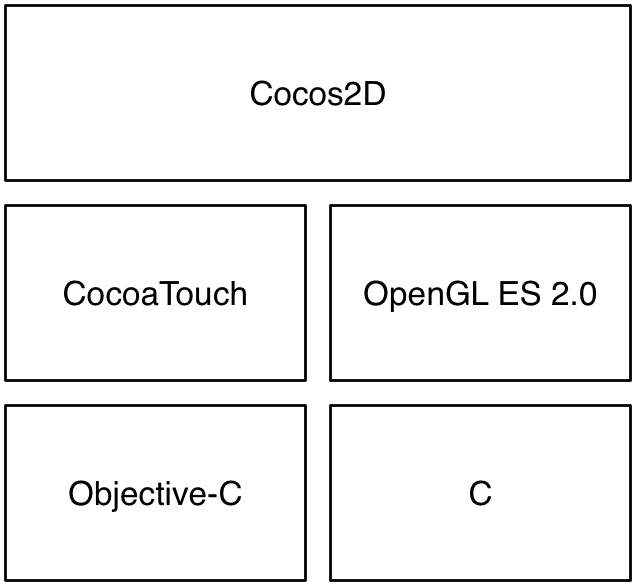
\includegraphics[width=120pt]{images/cocos2d/TechnologyStack.png}     
		\caption{Cocos2D Technology Stack}
\end{figure}

As a \cocos{} developer you define which scenes exist in your game, which
objects are part of these scenes and which size, position and appearance these
objects have and \cocos{} will use OpenGL to render the scene you have
described.

You have probably realized this already - when working with a 2D game engine for
the first time you will be introduced to a whole set of new terminology. Just as a framework to write desktop
applications knows the concept of windows, buttons and mouse clicks a 2D game
engine comes with its own set of terms and techniques. We will spent the next
sections discussing the important terms in detail.

\subsection{Scenes}
For explaining the important terms and concepts of \cocos{} I will use a top
down approach. First we will learn how games that use \cocos{} are structured.
On the highest level of structure we have a concept called \textit{scenes}. By default every scene in
\cocos{} is full-screen. This means for every screen in your game you will use
one scene.

Here's an example from the MakeGamesWithUs game \textit{Deep Sea Fury}:
% add image
You can see that the game consists of the start scene, the gameplay scene and
the game over scene.

A \cocos{} developer creates scenes by using the \ccscene{} class. Another
important \cocos{} class for scene handling is \ccdirector{}. The \ccdirector{}
class is responsible for deciding which scene is currently active in the game
(\cocos{} only allows one active scene at a time). Whenever a developer wants to
display a scene or transition between two scenes he needs to use the
\ccdirector{} class.

\subsection{Nodes}
\subsection{Scene Graphs}

\section{Introduction to \SB{}}
As of this writing SpriteBuilder itself is a very new tool, released in early
2014.

\subsection{The Editor}
\subsection{CCB Files}
\subsection{Publishing - How \SB{} and \xcode work together}
\subsection{How \SB{} and \cocos{}}
\subsection{Code Connections}

\section{A first \SB project} 